\section{Wprowadzenie}
W tej sekcji przedstawiono szczegółowy opis implementacji projektu, w tym wybór technologii, narzędzi programistycznych oraz środowiska, w którym został zrealizowany. Omówione zostaną również kluczowe aspekty techniczne, takie jak struktura bazy danych, architektura backendu i frontendu, a także proces testowania i napotkane problemy implementacyjne. Celem tej sekcji jest dostarczenie pełnego obrazu technicznego projektu oraz uzasadnienie wyboru poszczególnych rozwiązań technologicznych.


\section{Środowisko i narzędzia programistyczne}

\subsection{Środowisko programistyczne}
Do implementacji projektu wykorzystano następujące narzędzia i środowiska programistyczne:
\begin{itemize}
    \item \textbf{Visual Studio Code:} Środowisko programistyczne do tworzenia aplikacji internetowych w JavaScript i Python.
    \item \textbf{Git:} System kontroli wersji do zarządzania kodem źródłowym projektu.
    \item \textbf{MongoDB Atlas:} Usługa do hostowania bazy danych MongoDB w chmurze.
    \item \textbf{Flask:} Środowisko do tworzenia aplikacji webowych w Pythonie.
    \item \textbf{TypeScript:} Język programowania, który kompiluje się do JavaScriptu i dodaje typy danych w kodzie.

\end{itemize}
\subsection{Wybór technologii}
W trakcie realizacji projektu wykorzystano następujące technologie:
\begin{itemize}
    \item \textbf{Next.js:} Framework do tworzenia aplikacji internetowych w React, który oferuje wiele wbudowanych funkcji, takich jak routing, server-side rendering czy generowanie statyczne \cite{nextjs}.
    \item \textbf{Python:} Język programowania, który wykorzystałem do implementacji algorytmów przetwarzania języka naturalnego (NLP).
    \item \textbf{React Virtuoso:} Biblioteka do wirtualizacji list w aplikacjach internetowych.
    \item \textbf{Node.js:} Środowisko uruchomieniowe JavaScript, które pozwala na tworzenie aplikacji serwerowych.
    \item \textbf{MongoDB:} Baza danych NoSQL, która umożliwia przechowywanie danych w formacie JSON.
    \item \textbf{React.js:} Biblioteka do tworzenia interfejsów użytkownika w aplikacjach internetowych.
    \item \textbf{Shadcn:} Bibloteka gotowych komponentów do budowy interfejsu użytkownika w React.
    \item \textbf{Redux:} Biblioteka do zarządzania stanem aplikacji w React.
    \item \textbf{Prisma:} ORM do zarządzania bazą danych w Node.js.
    \item \textbf{Axios:} Biblioteka do wykonywania zapytań HTTP w JavaScript.
    \item \textbf{Tailwind CSS:} Narzędzie do tworzenia stylów CSS za pomocą gotowych klas, umożliwiające szybkie projektowanie responsywnych interfejsów.
\end{itemize}

\subsection{Opis technologii}
\subsubsection{Next.js}
Next.js to framework do tworzenia aplikacji internetowych w React, który oferuje wiele wbudowanych funkcji, takich jak routing, server-side rendering czy generowanie statyczne. Dzięki temu można tworzyć wydajne i skalowalne aplikacje internetowe, które są przyjazne dla SEO i łatwe w utrzymaniu. Next.js oferuje również wiele gotowych rozwiązań, takich jak automatyczne generowanie ścieżek, obsługa dynamicznych routów czy optymalizacja obrazów \cite{nextjs}. Dzięki temu można skupić się na tworzeniu funkcjonalności, zamiast martwić się o konfigurację i optymalizację aplikacji.
Kolejną istotną zaletą Next.js jest intuicyjny i wydajny system routingu oparty na strukturze plików. Ułatwia to organizację aplikacji i nawigację po niej, co jest kluczowe dla zachowania przejrzystości i spójności struktury. Next.js oferuje również uproszczone pobieranie danych oraz wsparcie dla różnych metod stylizacji, takich jak moduły CSS i Tailwind CSS, co pozwala na tworzenie estetycznego i responsywnego interfejsu użytkownika szybciej i łatwiej. Dodatkowo, framework zapewnia wsparcie dla TypeScript, co umożliwia tworzenie bezpiecznego i stabilnego kodu przy użyciu typów które nam podkreślą jeśli będziemy próbowali błędnie używac naszych funkcji lub zmiennych. Wszystkie te cechy czynią Next.js idealnym wyborem do stworzenia nowoczesnej i wydajnej aplikacji językowej.

\subsubsection{Python}
Python to język programowania, który wykorzystałem do implementacji algorytmów przetwarzania języka naturalnego (NLP). Python jest popularny w dziedzinie analizy danych i uczenia maszynowego, dzięki czemu można znaleźć wiele gotowych bibliotek i narzędzi do przetwarzania tekstu. W moim projekcie wykorzystałem biblioteki takie jak NLTK, spaCy czy TextBlob do lematyzacji, oznaczania części mowy i analizy sentymentu tekstu.

\subsubsection{React Virtuoso}
React Virtuoso to biblioteka do wirtualizacji list w aplikacjach internetowych. Umożliwia renderowanie długich list danych w sposób efektywny i wydajny, co przyczynia się do poprawy wydajności i płynności interfejsu użytkownika. Dzięki React Virtuoso można renderować tylko widoczne elementy i kilka dodatkowych poza obszarem.

\subsubsection{Node.js}
Node.js to środowisko uruchomieniowe JavaScript, które pozwala na tworzenie aplikacji serwerowych. Dzięki Node.js można pisać zarówno frontend, jak i backend w jednym języku programowania, co ułatwia rozwój i utrzymanie aplikacji. Node.js oferuje również wiele gotowych modułów i bibliotek, które ułatwiają tworzenie aplikacji internetowych, takich jak Express.js, Socket.io czy Mongoose.

\subsubsection{MongoDB}
Wybór bazy danych do aplikacji webowej ma ogromne znaczenie dla jej wydajności i skalowalności. W tym projekcie zdecydowano się na MongoDB Atlas, która jest objektową bazą danych typu NoSQL. MongoDB charakteryzuje się elastyczną strukturą danych, co pozwala na szybkie i efektywne przechowywanie oraz zarządzanie różnorodnymi danymi w formacie JSON. W projekcie baza danych została wykorzystana do przechowywania danych o użytkownikach, słowach do nauki, napisach oraz postępach w nauce.

\subsubsection{React.js}
React.js to biblioteka do tworzenia interfejsów użytkownika w aplikacjach internetowych. React.js oferuje wiele funkcji i narzędzi, które ułatwiają tworzenie interaktywnych i responsywnych interfejsów. Dzięki React.js można tworzyć komponenty UI, zarządzać stanem aplikacji i reagować na interakcje użytkownika w sposób efektywny i wydajny.

\subsubsection{Shadcn}
Shadcn to kolekcja komponentów, które można kopiować i wklejać do swoich aplikacji. Nie jest to biblioteka komponentów, którą można zainstalować jako zależność. Shadcn nie jest dostępny ani dystrybuowany przez npm (node package manager). Użytkownik wybiera potrzebne komponenty, kopiuje i wkleja kod do swojego projektu, a następnie dostosowuje go do swoich potrzeb. Kod jest własnością użytkownika. Shadcn może służyć jako odniesienie do budowy własnych bibliotek komponentów. do rozbudowy interfejsu użytkownika w React. Shadcn oferuje wiele gotowych rozwiązań, takich jak przyciski, formularze, tabele czy karty, które można łatwo dostosować do własnych potrzeb. Dzięki Shadcn można tworzyć interfejsy użytkownika w sposób szybki i efektywny, co przyczynia się do skrócenia czasu potrzebnego na rozwój aplikacji.





Jedną z kluczowych zalet MongoDB jest jej skalowalność. Baza ta umożliwia łatwe skalowanie poziome, co oznacza, że możemy dodawać nowe serwery do naszego klastra bazodanowego w miarę wzrostu ilości danych i liczby użytkowników. Jest to szczególnie ważne dla aplikacji edukacyjnych, które mogą szybko rosnąć w popularność i wymagać zwiększonej mocy obliczeniowej. Dzięki temu, nasza aplikacja będzie mogła obsługiwać rosnącą liczbę użytkowników bez utraty wydajności. Dodatkowo, MongoDB Atlas oferuje wsparcie dla replikacji danych, co zwiększa niezawodność i dostępność systemu. Funkcja replikacji zapewnia, że dane są automatycznie kopiowane na wiele serwerów, co chroni przed utratą danych i zapewnia ciągłość działania aplikacji. Dzięki tym funkcjom MongoDB Atlas jest idealnym wyborem dla naszej aplikacji, zapewniając jej wydajność, skalowalność i elastyczność w zarządzaniu danymi.

\section{Baza danych}


\section{Backend}
Backend aplikacji został zrealizowany przy użyciu dwóch technologii: Next.js oraz Flask. Każda z tych technologii pełni inną rolę w architekturze aplikacji, co pozwala na wykorzystanie ich mocnych stron w Flask został wykonany moduł pełniący funkcje lemmatyzacji i pos taggingu ponieważ modele NLP są tam bardzo mocno rozwinięte. W Next.js zostały wykonane endpointy do komunikacji z bazą danych oraz do obsługi logiki biznesowej aplikacji. Dzięki temu możliwe jest oddzielenie części serwerowej od frontendowej, co pozwala wykorzystać zalety szybkiego serwowania stron statycznych. Poniżej przedstawiono architekturę backendu z wykorzystaniem Next.js i Flask. Dodatkowo został wykorzystany moduł LibretTranslate do tłumaczenia maszynowego w aplikacji.

\subsubsection{Next.js}
Next.js jest wykorzystywany do obsługi części serwerowej aplikacji, która jest odpowiedzialna za renderowanie stron po stronie serwera (server-side rendering) oraz generowanie statycznych stron (static site generation). Dzięki temu aplikacja jest szybka i przyjazna dla SEO. Next.js umożliwia również łatwe zarządzanie ścieżkami strony które są wyświetlane w pasku url przeglądarki. Głównym celem w projekcie jest obsługa żądań HTTP, komunikacja z bazą danych MongoDB oraz wykonywanie operacji związanych z komunikacją z modułami NLP w Flask jak i modułem LibretTranslate do tłumaczenia maszynowego w aplikacji. Next.js oferuje również wsparcie dla różnych metod autoryzacji i uwierzytelniania, co zapewnia bezpieczeństwo aplikacji jak i szybkość działania i implementacji.
\subsection{Struktura backendu w Next.js}
Struktura backendu w Next.js została podzielona na kilka głównych katalogów, z których każdy odpowiada za określoną część aplikacji. Wszystkie pliki związane z budową backendu znajdują się w katalogu \texttt{src/app/api}, który zawiera następujące podkatalogi:

\begin{itemize}
    \item \textbf{auth:} Obsługuje autoryzację i uwierzytelnianie użytkowników.
    \item \textbf{captions:} Zajmuje się pobieraniem napisów z youtube.
    \item \textbf{hardWords:} Zajmuje się zarządzaniem trudnymi słowami.
    \item \textbf{profile:} Obsługuje aktualizacje profilu użytkownika.
    \item \textbf{sentence:} Zajmuje się aktualizacjami zdań.
    \item \textbf{signup:} Obsługuje rejestrację nowych użytkowników.
    \item \textbf{subtitles:} Zajmuje się zarządzaniem napisami do filmów.
\end{itemize}

\subsection{Struktura backendu w Flask}
Flask jest wykorzystywany do tworzenia API oraz logiki biznesowej aplikacji. Flask to lekki framework webowy dla Pythona, który umożliwia szybkie tworzenie i rozwijanie aplikacji webowych. W projekcie Flask jest odpowiedzialny za przetwarzanie żądań HTTP, oraz wykonywanie operacji związanych z przetwarzaniem języka naturalnego (NLP).
użyte do tego zostały modele:

\begin{lstlisting}[language=Python, caption=kod do importowania modeli NLP]
    nlp_de = spacy.load('de_core_news_md')
    nlp_ja = spacy.load('ja_core_news_md')
    nlp_en = spacy.load('en_core_web_md')
    nlp_pl = spacy.load('pl_core_news_md')
    
\end{lstlisting}

zostały one użyte do przetwarzania języka naturalnego w aplikacji. Dzięki temu możliwe jest lemmatyzacja i pos tagging słów w różnych językach. Do projektu zostały wykorzystane modele językowe dla języków: niemieckiego, japońskiego, angielskiego i polskiego. Reszta języków nie jest obsługiwana w aplikacji, ale można dodać nowe modele językowe w przyszłości.

\begin{lstlisting}[language=Python, caption=kod do obsługi lemmatyzacji i pos taggingu]
    @app.post("/nlp")
    async def analyze_text(request: AnalyzeTextRequest):
        word = request.word
        sourceLang = request.sourceLang
        doc = None
    
        if not sourceLang:
            raise HTTPException(status_code=400, detail="Source language is required")
        if sourceLang == 'de':
            doc = nlp_de(word)
        elif sourceLang == 'ja':
            doc = nlp_ja(word)
        elif sourceLang == 'en':
            doc = nlp_en(word)
        elif sourceLang == 'pl':
            doc = nlp_pl(word)
        elif sourceLang == 'auto':
            doc = nlp_de(word)
        else:
            raise HTTPException(status_code=400, detail=f"Source language is not currently used: {sourceLang}")
        
        tokens_with_pos = {'lemma': doc[0].lemma_, 'pos': doc[0].pos_}
        return {'result': tokens_with_pos}
\end{lstlisting}

% Funkcja \texttt{analyze_text} przyjmuje żądanie zawierające słowo oraz język źródłowy,
a następnie przetwarza tekst przy użyciu odpowiedniego modelu językowego. W przypadku braku określenia języka źródłowego lub podania nieobsługiwanego języka, zwracany jest odpowiedni komunikat błędu.
Wynikiem przetwarzania jest lemat naszego słowa oraz oznaczenie części mowy w obu przypadkach wybrane są te najbardziej prawdopobone w przetworzonym dokumencie który zwrócił model NLP.


\subsection{LibretTranslate}
LibretTranslate to otwartoźródłowy system tłumaczenia maszynowego, który umożliwia tłumaczenie tekstów pomiędzy różnymi językami. W projekcie został wykorzystany do tłumaczenia tekstów w aplikacji, co pozwala na obsługę użytkowników mówiących różnymi językami. LibretTranslate wspiera wiele języków, co czyni go wszechstronnym narzędziem do tłumaczeń.

\subsubsection{Integracja LibretTranslate}
Integracja LibretTranslate w aplikacji została zrealizowana poprzez stworzenie funkcji w Next.js, która komunikuje się z API LibretTranslate. Dzięki temu możliwe jest wysyłanie napisów do przetłumaczenia oraz odbieranie przetłumaczonych wyników bezpośrednio w aplikacji. Poniżej przedstawiono przykładowy kod obsługujący tłumaczenie napisów za pomocą LibretTranslate:

\begin{lstlisting}[language=JavaScript, caption=Przykładowy kod integracji LibretTranslate w Next.js]
import axios from 'axios';
export default async function translateText(req, res) {
    async function translateSubtitleData(subtitleData: SubtitleData[], targetLang: string) {
    try {
        const texts = subtitleData.map(subtitle => subtitle?.text);
        const response = await axios.post("http://127.0.0.1:5000/translate", {
            q: texts,
            source: "auto" ,
            target: targetLang || "en",
            format: "text"
        });
        let detectedLanguage = "auto";
        if(response.data.detectedLanguage[0].language){
            detectedLanguage = response.data.detectedLanguage[0].language;
        }
        return {
            translatedSubtitleData: response.data.translatedText,
            detectedLanguage
        };
    } catch (error) {
        console.error('Error translating subtitles:', error);
        throw new Error('Failed to translate subtitles');
    }
}
}
\end{lstlisting}

Funkcja \texttt{translateSubtitleData} przyjmuje dane napisów oraz język docelowy, a następnie wysyła zapytanie do API LibretTranslate w celu przetłumaczenia tekstu. Odpowiedź zawiera przetłumaczone napisy oraz wykryty język źródłowy, co pozwala na dalsze przetwarzanie danych w aplikacji.
\section{Frontend}
\subsection{Struktura projektu}
Struktura projektu została podzielona na kilka głównych katalogów, z których każdy odpowiada za określoną część aplikacji. Wszystkie pliki związane z budową aplikacji znajdują się w katalogu \texttt{src}, który zawiera następujące podkatalogi:
\begin{itemize}
    \item \textbf{app:} Zawiera wszystkie strony aplikacji, które są renderowane przez Next.js. Każda strona jest reprezentowana przez plik JavaScript, który eksportuje komponent React.
    \item \textbf{app/home:} Jest to strona główna aplikacji, która wyświetla różne sekcje, takie jak podstrona napisów, podstrona do nauki czy podstrona statystyk użytkownika, razem z resztą podstron wszystkie są zawarte w tym katalogu home poza stroną authoryzacji.
    \item \textbf{app/auth:} Jest to strona autoryzacji, która wyświetla formularze logowania i rejestracji użytkownika.
    \item \textbf{app/api:} Zawiera pliki z funkcjami, które obsługują zapytania API do serwera. W projekcie wykorzystano bibliotekę axios do wykonywania zapytań HTTP.
    \item \textbf{styles:} Zawiera pliki CSS, które definiują styl aplikacji. W projekcie wykorzystano ją do tworzenia domyślnych styli aplikacji i styli motywów które dają kontrole nad kolorami i zaokrągleniem obramowań.
    \item \textbf{components:} Zawiera wszystkie komponenty interfejsu użytkownika, takie jak przyciski, formularze, tabele czy karty.
    \item \textbf{hooks:} Zawiera pliki z hookami, które są wykorzystywane w różnych częściach aplikacji. W projekcie wykorzystano hooki do zarządzania stanem, efektami ubocznymi i logiką aplikacji.
    \item \textbf{providers:} Zawiera pliki z providermi, które są wykorzystywane do dostarczania kontekstów i hooków do komponentów aplikacji.
    \item \textbf{lib:} Zawiera pliki z funkcjami pomocniczymi, które są wykorzystywane w różnych częściach aplikacji. W projekcie znajduje się tam głównie kod związany z Redux, który jest używany do zarządzania stanem aplikacji.
    \item \textbf{styles:} Zawiera pliki CSS, które definiują styl aplikacji. W projekcie wykorzystano bibliotekę styled-components do tworzenia stylów w JavaScript.
    \item \textbf{types:} Zawiera pliki z typami, które definiują struktury danych w aplikacji. W projekcie wykorzystano TypeScript do dodawania typów danych w kodzie. są one domyślnie w plikach .d.ts które pozwalają na dodanie typów do plików JavaScript bez podawania scieżki działają one automatycznie.
\end{itemize}

poza tym katalogiem znajdują się również pliki konfiguracyjne, takie jak \texttt{package.json}, \texttt{tsconfig.json} czy \texttt{.env}, które definiują zależności, ustawienia TypeScript i zmienne środowiskowe aplikacji. Struktura projektu została zaprojektowana w taki sposób, aby była czytelna i łatwa w utrzymaniu, co przyczynia się do szybszego rozwoju aplikacji i łatwiejszej nawigacji.

I pozostałe katalogi w projekcie. Katalog \texttt{public} zawiera pliki statyczne, takie jak obrazy, ikony czy pliki konfiguracyjne, które są dostępne publicznie i mogą być bezpośrednio serwowane przez serwer. Katalog \texttt{prisma} zawiera pliki konfiguracyjne i schematy bazy danych używane przez Prisma ORM do zarządzania bazą danych. Prisma umożliwia łatwe definiowanie modeli danych i wykonywanie zapytań do bazy danych. Katalog \texttt{node\_modules} zawiera wszystkie zainstalowane zależności projektu, które są pobierane za pomocą npm (Node Package Manager). Katalog ten jest automatycznie generowany i zarządzany przez npm na podstawie pliku \texttt{package.json}.

\subsection{Panel nauki Fiszek}
\begin{figure}[H]
    \centering
    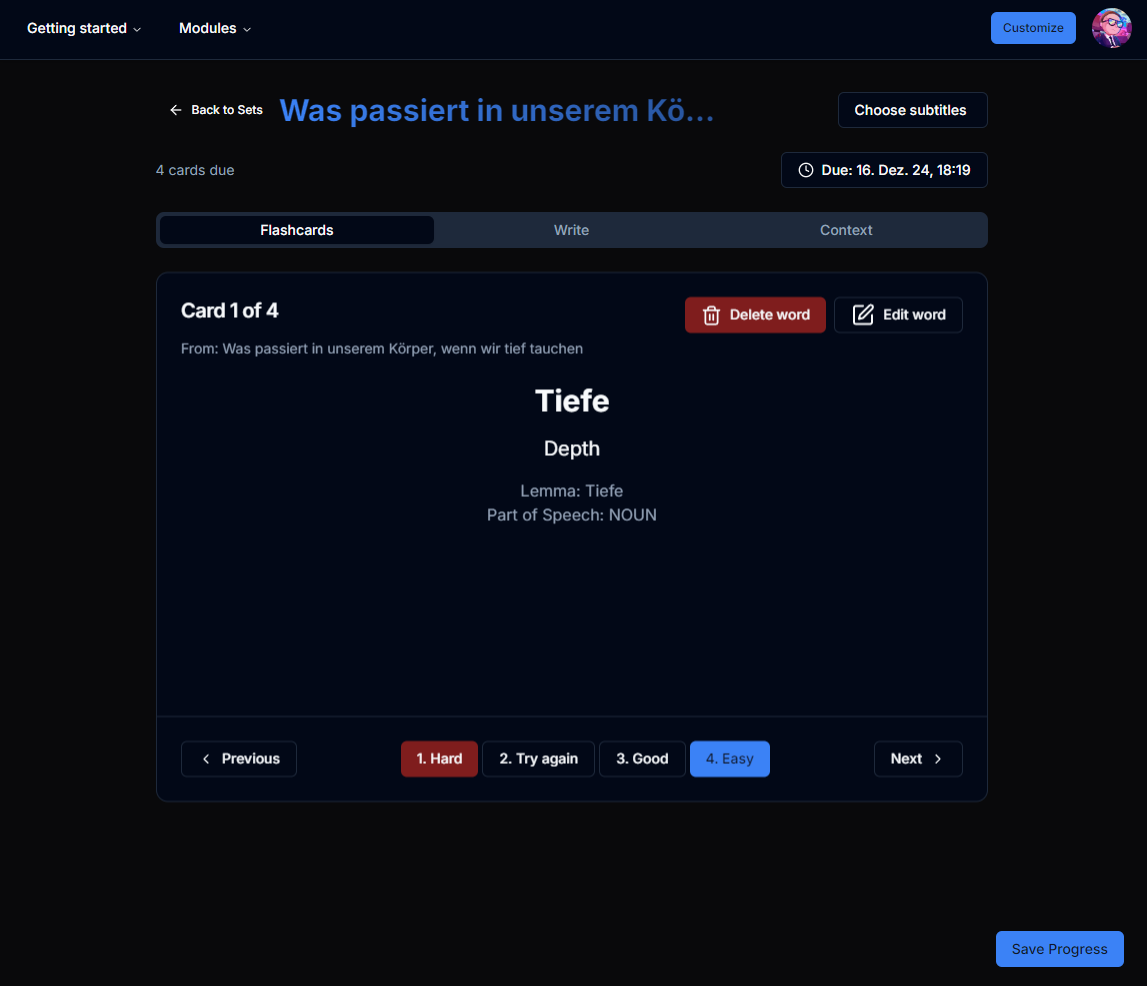
\includegraphics[width=1\textwidth]{IMAGE/FlashcardsLearn.png}
    \caption{Panel nauki fiszek}
    \label{fig:FlashcardsLearn}
\end{figure}

Panel nauki w aplikacji został zaprojektowany w oparciu o system fiszek oraz system powtórek oparty na algorytmie SRS (Space Repetition System). System fiszek umożliwia użytkownikom naukę nowych słów i zwrotów poprzez prezentowanie im kart z słowami i tłumaczeniami. Użytkownik może ocenić swoją znajomość danego słowa, co wpływa na to czy słowo przejdzie dalej czy nasze powtórki zostaną cofnięte.

\subsection*{System powtórek SRS}

System SRS jest algorytmem, który optymalizuje proces nauki poprzez dostosowanie interwałów powtórek do indywidualnych potrzeb użytkownika. W praktyce oznacza to, że słowa, które użytkownik zna dobrze, będą pojawiać się rzadziej, natomiast te, które sprawiają trudności, będą powtarzane częściej. Dzięki temu użytkownik może efektywnie zarządzać swoim czasem nauki i skupić się na materiałach, które wymagają większej uwagi.

W panelu nauki użytkownik ma dostęp do różnych zestawów fiszek, które mogą być tworzone ręcznie lub generowane automatycznie na podstawie jego postępów i preferencji. Każda fiszka zawiera słowo lub zwrot w języku obcym oraz jego tłumaczenie lub definicję. Użytkownik może również edytowac fiszki, dodać tłumaczenie lub usuwać niepotrzebne lub niepoprawne informacje.

Dzięki zastosowaniu systemu SRS, panel nauki w aplikacji zapewnia skuteczną metodę nauki języka, która pozwala na osiąganie lepszych wyników w krótszym czasie. System automatycznie dostosowuje interwały powtórek na podstawie wyników użytkownika, co optymalizuje proces nauki bez konieczności ręcznej ingerencji.

\subsection{Wirtualizacja List}
Wirtualizacja listy w aplikacjach internetowych to technika, która optymalizuje renderowanie długich list danych. Bez niej aplikacja renderuje wszystkie elementy listy na raz, co może prowadzić do problemów z wydajnością, zwłaszcza gdy lista jest duża. Virtualizacja polega na renderowaniu jedynie tych elementów, które aktualnie są widoczne w przeglądarce użytkownika, dzięki czemu zużycie zasobów jest minimalne, a aplikacja działa płynniej. Bez wirtualizacji listy, użytkownik mógłby doświadczać opóźnień w interakcji z interfejsem, tym większych im dłuższa lista danych przy 2 tysiącach wierszy opóźnienie stawało się uciążliwe ponieważ czekało sie pare sekund na reakcje interfejsu listy i pokazanie okna dodawania trudnych słów do systemu.

\subsection*{Mechanizm działania wirtualizacji listy}
\begin{itemize}
    \item \textbf{Obserwacja widocznych elementów:} Komponent śledzi pozycję widoku użytkownika w liście. Renderowane są tylko te elementy, które mieszczą się w aktualnie widocznym obszarze (viewport) oraz kilka dodatkowych elementów „na zapas” wokół tego obszaru.
    \item \textbf{Renderowanie na żądanie:} Gdy użytkownik przewija listę, niewidoczne elementy są dynamicznie usuwane z DOM-u, a nowe – wczytywane na ich miejsce.
    \item \textbf{Stała wysokość elementów (lub szacowana):} Dla prawidłowego działania, komponent wirtualizujący często wymaga, aby elementy listy miały stałą lub przynajmniej przewidywalną wysokość. Dzięki temu może łatwo obliczać, które elementy powinny być aktualnie wyświetlane.
    \item \textbf{Oszczędność zasobów:} Dzięki renderowaniu tylko niewielkiej liczby elementów, zmniejsza się zużycie pamięci i obciążenie procesora, co prowadzi do szybszego działania aplikacji.
\end{itemize}
\subsection*{Przykładowy kod JavaScript}
Poniżej przedstawiono przykładowy kod tabeli Tanstack, który ilustruje operowanie na wierszach tabeli, takie jak śledzenie aktualnego do filmu wiersza napisów. Wiersz jest automatycznie przewijany do środkowego obszaru widocznego dla użytkownika, co ułatwia śledzenie napisów w czasie rzeczywistym. A index wiersza jest wybierany na podstawie czasu odtwarzania filmu, wybierany jest pierwszy wiersz na początek a potem przechodzi się na kolejny jeśli czas przekroczy wartość czasu w sekundach kolejnego wiersza.

\begin{lstlisting}[language=JavaScript, caption=Tablica Tanstack do wirtualizacji listy]
    export function DataTable<TData, TValue>({ captions, height }: { captions: Caption[], height: string }) {
        const [sorting, setSorting] = useState<SortingState>([]);
        const [currentIndex, setCurrentIndex] = useState<number>(0);
        const playedSeconds = useSelector((state: any) => state.subtitle.playedSeconds);
        const autoScrollEnabled = useSelector((state: any) => state.subtitle.autoScrollEnabled);
        const tableRef = useRef<TableVirtuosoHandle>(null);
        const table = useReactTable({
            data: captions,
            columns: columns,
            state: {
                sorting,
            },
            onSortingChange: setSorting,
            getCoreRowModel: getCoreRowModel(),
            getSortedRowModel: getSortedRowModel(),
        });
        const { rows } = table.getRowModel()
        useEffect(() => {
            if (rows.length > 0) {
                let newIndex = -1;
                for (let i = 0; i < rows.length; i++) {
                    const row = rows[i];
                    const startTime = row.original.start ?? 0;
                    const nextStartTime = rows[i + 1]?.original.start ?? Infinity;
                    if (playedSeconds >= startTime && playedSeconds < nextStartTime) {
                        newIndex = i;
                        break;
                    }
                }

                if (newIndex === -1) {
                    newIndex = 0;
                }
                setCurrentIndex(newIndex);
                if (autoScrollEnabled && tableRef.current && newIndex !== -1) {
                    tableRef.current.scrollToIndex({
                        index: newIndex,
                        align: "center",
                        behavior: "smooth",
                    });
                }
            }
        }, [playedSeconds, rows, autoScrollEnabled]);
\end{lstlisting}

\subsection*{Dlaczego React Virtuoso}
React Virtuoso jest biblioteką do wirtualizacji list, która znacznie upraszcza implementację tego mechanizmu w React. Automatycznie obsługuje:
\begin{itemize}
    \item \textbf{Przewijanie:} Zajmuje się wykrywaniem widocznych elementów, reagując na przewijanie użytkownika.
    \item \textbf{Niestandardowe wysokości elementów:} Obsługuje zarówno stałe, jak i zmienne wysokości elementów, co czyni go bardziej elastycznym.
    \item \textbf{Lazy loading:} Umożliwia ładowanie danych w locie, co jest kluczowe dla dużych list z elementami, które mogą być dynamicznie ładowane z serwera.
\end{itemize}

\subsection*{Zastosowania}
Virtualizacja listy jest szczególnie przydatna w przypadku:
\begin{itemize}
    \item \textbf{Długich list:} Kiedy lista zawiera setki lub tysiące elementów.
    \item \textbf{Aplikacji mobilnych:} Gdzie zasoby są ograniczone i każda optymalizacja wydajności jest istotna.
    \item \textbf{Interfejsów użytkownika z dużą ilością dynamicznych danych:} Takich jak portale społecznościowe, aplikacje e-commerce czy dashboardy.
\end{itemize}

\subsection*{Wady}
Mimo licznych zalet, wirtualizacja listy ma również pewne wady:
\begin{itemize}
    \item \textbf{Złożoność implementacji:} Wprowadzenie wirtualizacji może wymagać dodatkowego kodu i konfiguracji, co może zwiększyć złożoność projektu.
    \item \textbf{Problemy z dostępnością:} Renderowanie dynamiczne może wpływać na narzędzia do czytania ekranu i inne technologie wspomagające, co może utrudniać dostępność aplikacji.
\end{itemize}

Wykorzystanie React Virtuoso przyczyniło się do poprawy wydajności i płynności interfejsu użytkownika  aplikacji, co miało kluczowe znaczenie dla zadowolenia użytkowników i jakości doświadczenia użytkownika.

\section{Problemy implementacyjne}
\subsection{Wirtualizacja List}
Wirtualizacja listy w aplikacjach internetowych to technika, która optymalizuje renderowanie długich list danych. Bez niej aplikacja renderuje wszystkie elementy listy na raz, co może prowadzić do problemów z wydajnością, zwłaszcza gdy lista jest duża. Virtualizacja polega na renderowaniu jedynie tych elementów, które aktualnie są widoczne w przeglądarce użytkownika, dzięki czemu zużycie zasobów jest minimalne, a aplikacja działa płynniej. Bez wirtualizacji listy, użytkownik mógłby doświadczać opóźnień w interakcji z interfejsem, tym większych im dłuższa lista danych przy 2 tysiącach wierszy opóźnienie stawało się uciążliwe ponieważ czekało sie pare sekund na reakcje interfejsu listy i pokazanie okna dodawania trudnych słów do systemu.


\subsection*{Jak działa wirtualizacja listy}
\begin{itemize}
    \item \textbf{Obserwacja widocznych elementów:} Komponent śledzi pozycję widoku użytkownika w liście. Renderowane są tylko te elementy, które mieszczą się w aktualnie widocznym obszarze (viewport) oraz kilka dodatkowych elementów „na zapas” wokół tego obszaru.
    \item \textbf{Renderowanie na żądanie:} Gdy użytkownik przewija listę, niewidoczne elementy są dynamicznie usuwane z DOM-u, a nowe – wczytywane na ich miejsce.
    \item \textbf{Stała wysokość elementów (lub szacowana):} Dla prawidłowego działania, komponent wirtualizujący często wymaga, aby elementy listy miały stałą lub przynajmniej przewidywalną wysokość. Dzięki temu może łatwo obliczać, które elementy powinny być aktualnie wyświetlane.
    \item \textbf{Oszczędność zasobów:} Dzięki renderowaniu tylko niewielkiej liczby elementów, zmniejsza się zużycie pamięci i obciążenie procesora, co prowadzi do szybszego działania aplikacji.
\end{itemize}
\subsection*{Przykładowy kod JavaScript}
Poniżej przedstawiono przykładowy kod tabeli Tanstack, który ilustruje operowanie na wierszach tabeli, takie jak śledzenie aktualnego do filmu wiersza napisów. Wiersz jest automatycznie przewijany do środkowego obszaru widocznego dla użytkownika, co ułatwia śledzenie napisów w czasie rzeczywistym. A index wiersza jest wybierany na podstawie czasu odtwarzania filmu, wybierany jest pierwszy wiersz na początek a potem przechodzi się na kolejny jeśli czas przekroczy wartość czasu w sekundach kolejnego wiersza.

\begin{lstlisting}[language=JavaScript, caption=Tablica Tanstack do wirtualizacji listy]
    export function DataTable<TData, TValue>({ captions, height }: { captions: Caption[], height: string }) {
        const [sorting, setSorting] = useState<SortingState>([]);
        const [currentIndex, setCurrentIndex] = useState<number>(0);
        const playedSeconds = useSelector((state: any) => state.subtitle.playedSeconds);
        const autoScrollEnabled = useSelector((state: any) => state.subtitle.autoScrollEnabled);
        const tableRef = useRef<TableVirtuosoHandle>(null);
        const table = useReactTable({
            data: captions,
            columns: columns,
            state: {
                sorting,
            },
            onSortingChange: setSorting,
            getCoreRowModel: getCoreRowModel(),
            getSortedRowModel: getSortedRowModel(),
        });
        const { rows } = table.getRowModel()
        useEffect(() => {
            if (rows.length > 0) {
                let newIndex = -1;
                for (let i = 0; i < rows.length; i++) {
                    const row = rows[i];
                    const startTime = row.original.start ?? 0;
                    const nextStartTime = rows[i + 1]?.original.start ?? Infinity;
                    if (playedSeconds >= startTime && playedSeconds < nextStartTime) {
                        newIndex = i;
                        break;
                    }
                }

                if (newIndex === -1) {
                    newIndex = 0;
                }
                setCurrentIndex(newIndex);
                if (autoScrollEnabled && tableRef.current && newIndex !== -1) {
                    tableRef.current.scrollToIndex({
                        index: newIndex,
                        align: "center",
                        behavior: "smooth",
                    });
                }
            }
        }, [playedSeconds, rows, autoScrollEnabled]);
\end{lstlisting}

\subsection*{Dlaczego React Virtuoso}
React Virtuoso jest biblioteką do wirtualizacji list, która znacznie upraszcza implementację tego mechanizmu w React. Automatycznie obsługuje:
\begin{itemize}
    \item \textbf{Przewijanie:} Zajmuje się wykrywaniem widocznych elementów, reagując na przewijanie użytkownika.
    \item \textbf{Niestandardowe wysokości elementów:} Obsługuje zarówno stałe, jak i zmienne wysokości elementów, co czyni go bardziej elastycznym.
    \item \textbf{Lazy loading:} Umożliwia ładowanie danych w locie, co jest kluczowe dla dużych list z elementami, które mogą być dynamicznie ładowane z serwera.
\end{itemize}

\subsection*{Zastosowania}
Virtualizacja listy jest szczególnie przydatna w przypadku:
\begin{itemize}
    \item \textbf{Długich list:} Kiedy lista zawiera setki lub tysiące elementów.
    \item \textbf{Aplikacji mobilnych:} Gdzie zasoby są ograniczone i każda optymalizacja wydajności jest istotna.
    \item \textbf{Interfejsów użytkownika z dużą ilością dynamicznych danych:} Takich jak portale społecznościowe, aplikacje e-commerce czy dashboardy.
\end{itemize}

\subsection*{Wady}
Mimo licznych zalet, wirtualizacja listy ma również pewne wady:
\begin{itemize}
    \item \textbf{Złożoność implementacji:} Wprowadzenie wirtualizacji może wymagać dodatkowego kodu i konfiguracji, co może zwiększyć złożoność projektu.
    \item \textbf{Problemy z dostępnością:} Renderowanie dynamiczne może wpływać na narzędzia do czytania ekranu i inne technologie wspomagające, co może utrudniać dostępność aplikacji.
\end{itemize}

Wykorzystanie React Virtuoso przyczyniło się do poprawy wydajności i płynności interfejsu użytkownika  aplikacji, co miało kluczowe znaczenie dla zadowolenia użytkowników i jakości doświadczenia użytkownika.

\subsection{Przetwarzanie języka naturalnego (NLP)}
W pracy inżynierskiej zastosowano techniki lematyzacji oraz oznaczania części mowy (POS tagging) w ramach przetwarzania języka naturalnego (NLP). Obie te techniki odegrały kluczową rolę w analizie tekstu i umożliwiły bardziej precyzyjne przetwarzanie danych z napisów, przy zapisywaniu wybranych przez użytkownika słów do nauki, lub przy wyświetlaniu częstości występowania słów w napisach \cite{NLPforNLP}.

\subsection*{Lematyzacja}
Proces lematyzacji polega na sprowadzaniu różnych form gramatycznych wyrazów do ich podstawowej formy, zwanej lematem. Dzięki temu możliwe jest ujednolicenie wyrazów, które w zależności od kontekstu występują w różnych odmianach gramatycznych. Przykładowo, formy takie jak "chodzę", "chodził" czy "chodziliśmy" są sprowadzane do podstawowej formy "chodzić". Umożliwia to bardziej spójne analizowanie tekstów i wyciąganie wniosków na temat ich zawartości, np. poprzez obliczanie częstotliwości występowania poszczególnych słów \cite{NLPforNLP}.

\subsection*{POS Tagging (oznaczanie części mowy)}
Drugą techniką było oznaczanie części mowy, czyli przypisywanie każdemu słowu w tekście odpowiedniej etykiety gramatycznej (rzeczownik, czasownik, przymiotnik itd.)  \cite{NLPforNLP}. Dzięki temu możliwe było lepsze zrozumienie struktury zdań oraz funkcji słów w kontekście. Oznaczanie części mowy okazało się kluczowe w procesie analizy tekstu, umożliwiając podział słów na kategorie zależne od ich funkcji gramatycznej. W przyszłości może to być przydatne do tworzenia funkcji umożliwiających użytkownikom wybór nauki określonych kategorii słów, takich jak czasowniki czy przymiotniki itd.







